\documentclass{article}

\usepackage[nonatbib]{nips_2017}

\usepackage[utf8]{inputenc}         % allow utf-8 input
\usepackage[T1]{fontenc}            % use 8-bit T1 fonts
\usepackage{hyperref}               % hyperlinks
\usepackage{url}                    % simple URL typesetting
\usepackage{booktabs}               % professional-quality tables
\usepackage{amsfonts}               % blackboard math symbols
\usepackage{amsmath,amsthm,amssymb} % more math symbols
\usepackage{nicefrac}               % compact symbols for 1/2, etc.
\usepackage{microtype}              % microtypography

\usepackage{pdfpages}
\usepackage{graphicx}
\usepackage{subcaption}
\usepackage[export]{adjustbox}
\graphicspath{{./Figures/}}
\usepackage{float}

\usepackage{biblatex}
\addbibresource{ref.bib}

\usepackage[colorinlistoftodos]{todonotes}

\title{ECE 532: Final Project}

%----------------------------------------------------------------------------------------
%	DOCUMENT
%----------------------------------------------------------------------------------------

\begin{document}

\maketitle

%----------------------------------------------------------------------------------------
%	ABSTRACT
%----------------------------------------------------------------------------------------
\begin{abstract}
    In this project, the authors consider the \href{https://www.kaggle.com/c/mlsp-2014-mri}{MLSP 2014 Schizophrenia Classification Challenge} dataset and perform standard analysis techniques. The authors then present their findings, and finally, give observations drawn from their results.
\end{abstract}
\raggedbottom % stops vertical justification

%----------------------------------------------------------------------------------------
%	INTRODUCTION
%----------------------------------------------------------------------------------------
\section{Introduction}
The dataset provided by the Kaggle challenge contains testing sets and training sets for two features; Functional Network Connectivity (FNC) and Source-Based Morphometry (SBM) (more information on these can be found on the challenge page). In this project, only the FNC feature is considered. The objective of the challenge is to classify (as correctly as possible) individuals in the testing set who suffer from schizophrenia. Because the testing set data was not labelled (effectively making it useless for the purposes of this project), the given training set was randomly partitioned into two sets, an effective training set and a testing set (which will henceforth be referred to as the training set and testing set).

Note that the training set contains only 85 labelled samples, therefore after splitting it into an effective training set and testing set, the training set contained 72 samples, and the testing set contained 13 samples. Success was measured as the number of samples in the testing set that had predicted labels that matched the known and given labels. 

The objective of this project will be to answer the following: Which fundamental technique best classifies the test data?


Several methods at classification were made, and they are covered in full in the next section. The results of the analyses are also covered in the next section, followed by a discussion. This ends with a conclusion in the final section.

%----------------------------------------------------------------------------------------
%	ANALYSIS TECHNIQUES and RESULTS
%----------------------------------------------------------------------------------------
\section{Analysis Techniques and Results}
In this section, several techniques of classification are implemented. A brief discussion of implementation details are given, and results are either shown or stated.

\subsection{Singular Value Decomposition (SVD) for Principal Component Analysis (PCA)}
PCA was performed on the entire dataset. The idea was that this would highlight the two most important basis vectors that classify the data best, but this resulted in a solution that was not useful; there was no obvious separation between the healthy patients and the sufferers of schizophrenia. However, research into this led to the analysis in the next subsection.
\begin{figure}[H]
    \centering
    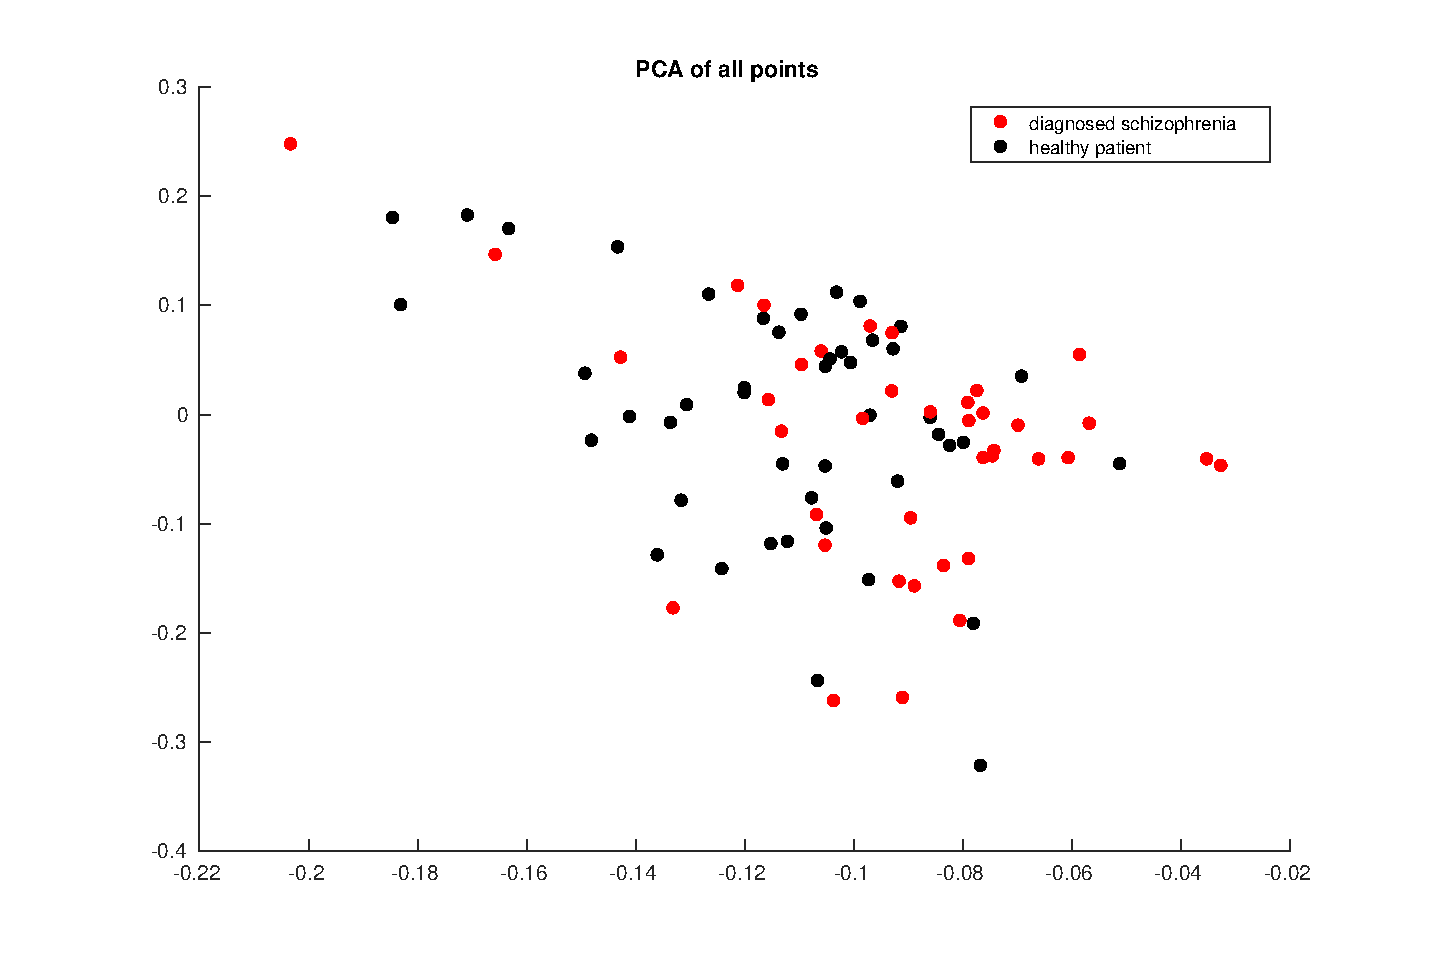
\includegraphics[width = \textwidth]{PCA.eps}
    \caption{PCA}
\end{figure}

\begin{figure}[H]
    \begin{subfigure}{0.5\textwidth}
        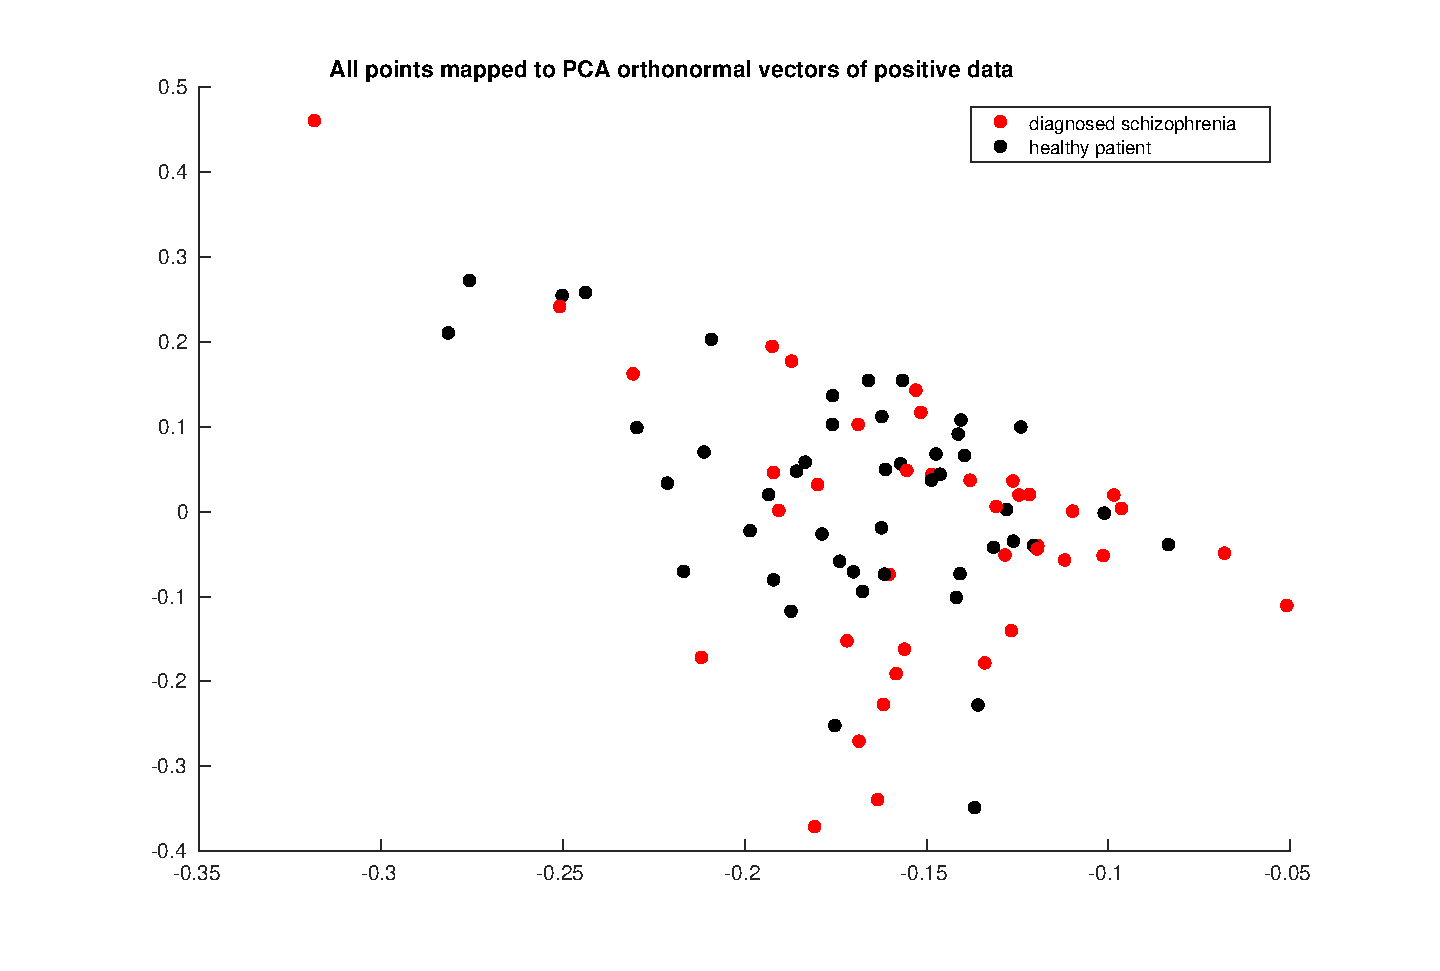
\includegraphics[width=0.9\linewidth, height=5cm]{Figures/PCApos.eps} 
        \caption{Using PCA orthonormal vectors of positive data}
    \end{subfigure}
    \begin{subfigure}{0.5\textwidth}
        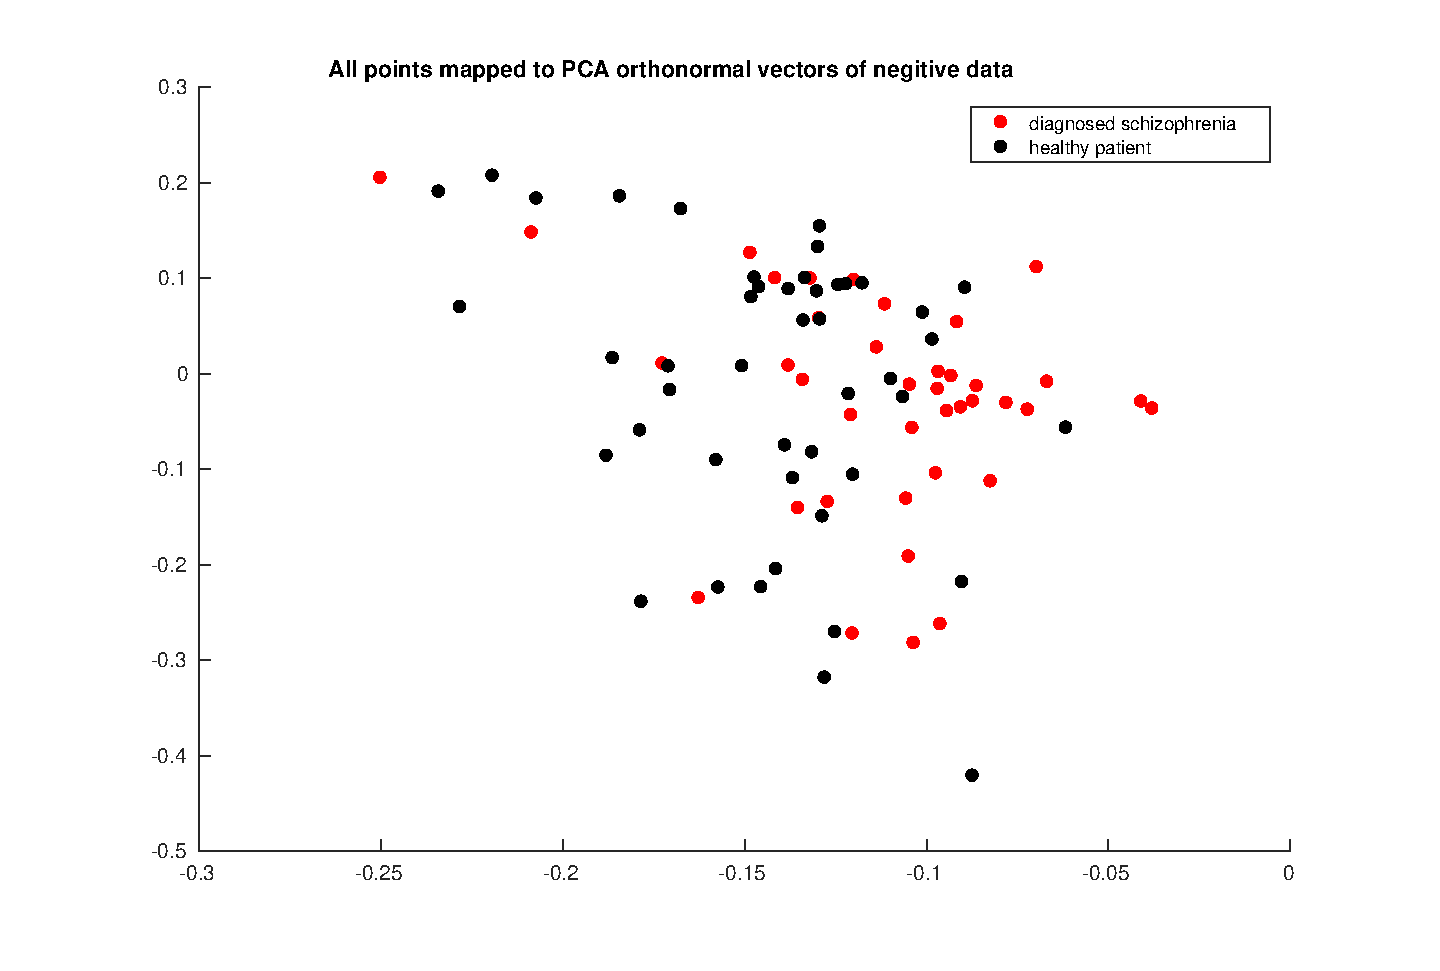
\includegraphics[width=0.9\linewidth, height=5cm]{Figures/PCAneg.eps}
        \caption{Using PCA orthonormal vectors of negative data}
    \end{subfigure}
 
    \caption{Point mappings with positive and negative data}
\end{figure}


\subsection{Singular Value Decomposition (SVD) for Linear Discriminant Analysis (LDA)}
In an attempt to apply Principal Component Analysis (PCA), research suggested an attempt at Linear Discriminant Analysis \cite{SebastianRaschka2014}. After implementing LDA, applying this once to the FNC training set, a clearly separable line formed of the two classes was achieved. By using the weight vector that produced this, using this weight vector to produce the basis vector associated with it, and then finding the residual of the training set with the original training data, LDA was performed once more. This had the effect of producing a second vector of weights which would result in a second basis vector. Another repeat of this was attempted (to see if a third basis vector would have much impact), but the norm of the resulting weight vector was small, meaning that the corresponding basis vector had little contribution to the overall classification. The results are shown below.

\begin{figure}[H]
    \begin{subfigure}{0.5\textwidth}
        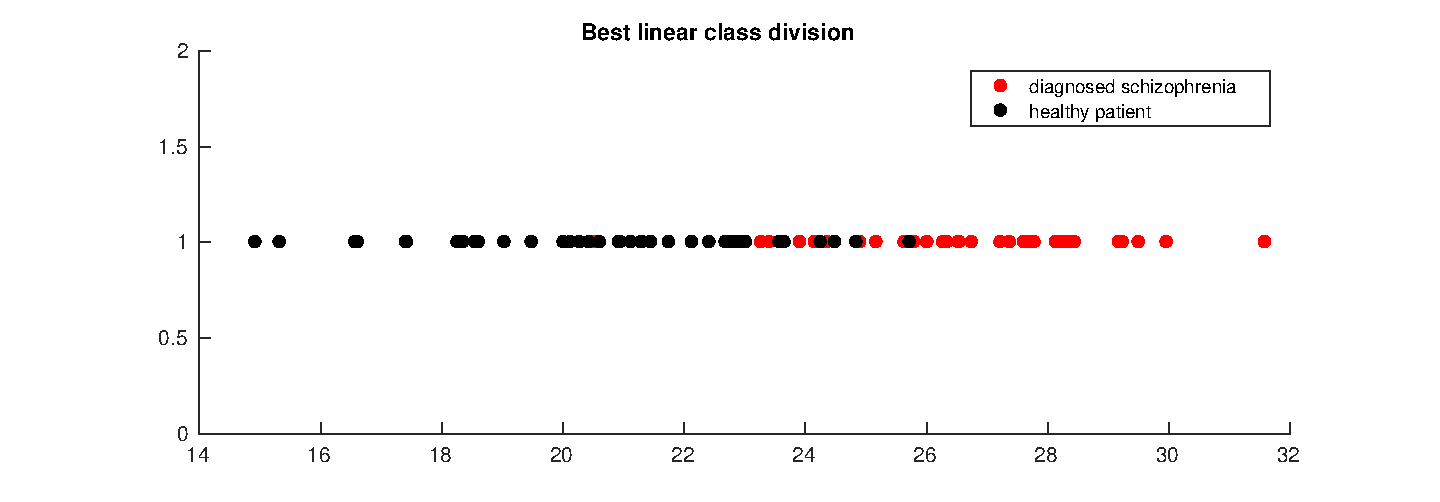
\includegraphics[width=0.9\linewidth, height=4cm]{Figures/LDA1D.eps} 
        \caption{Best linear separation on training data}
    \end{subfigure}
    \begin{subfigure}{0.5\textwidth}
        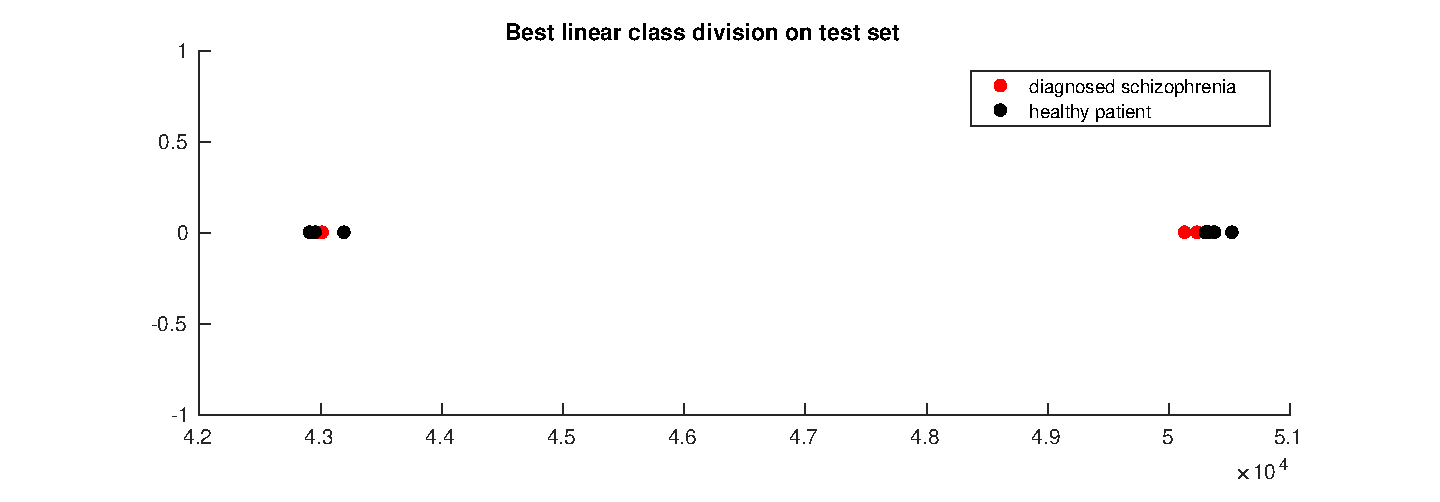
\includegraphics[width=0.9\linewidth, height=4cm]{Figures/LDA1DTest.eps}
        \caption{Best linear separation on testing data}
    \end{subfigure}
 
    \caption{1D LDA}
\end{figure}
\begin{figure}[H]
    \begin{subfigure}{0.5\textwidth}
        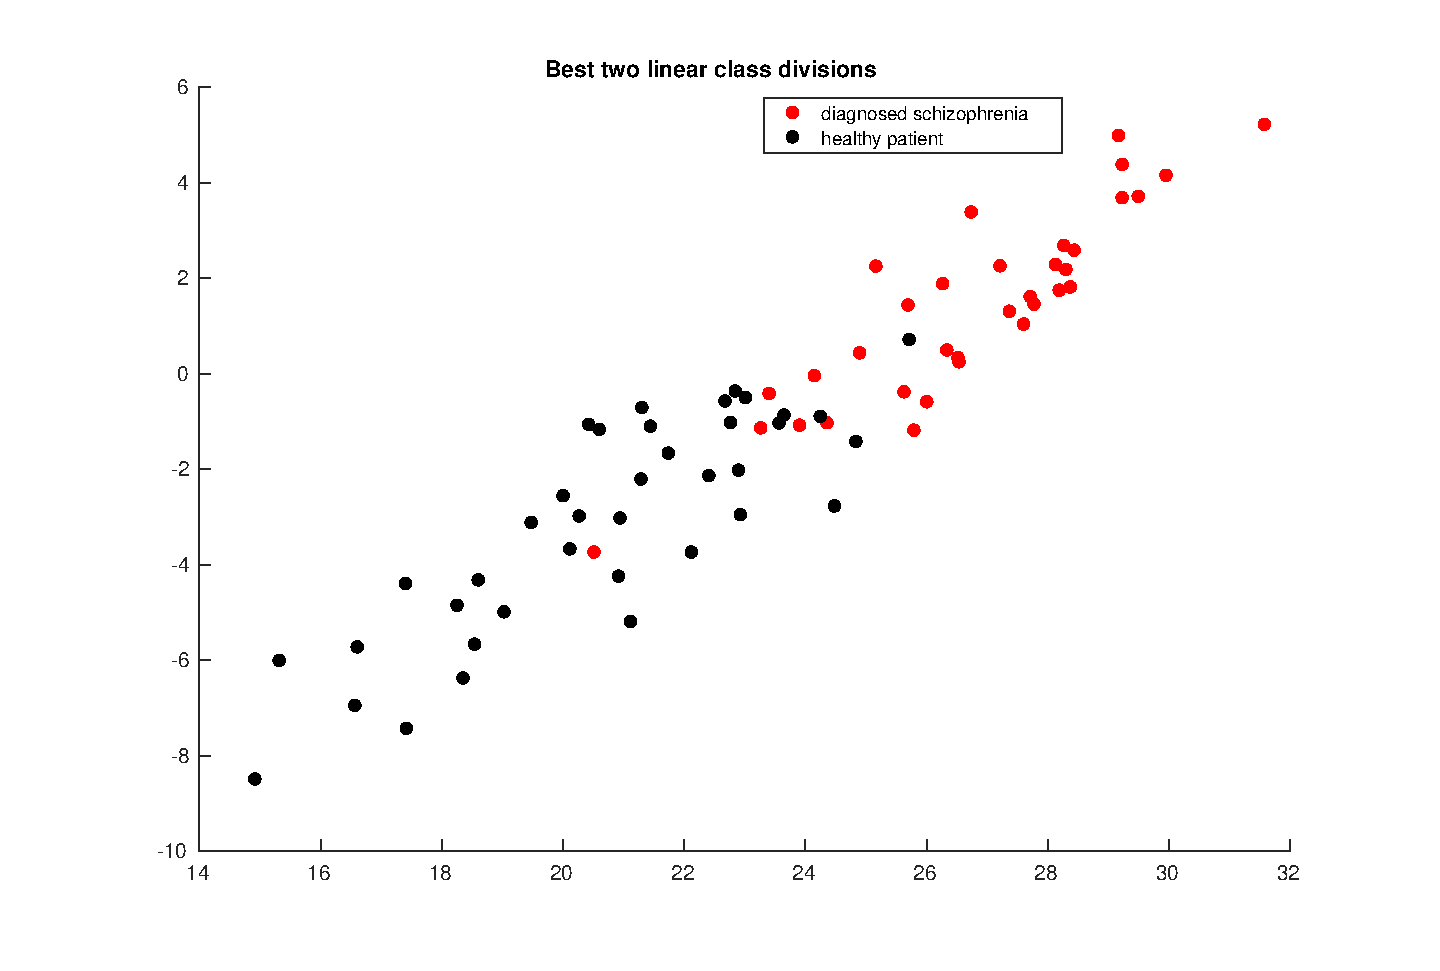
\includegraphics[width=0.9\linewidth, height=4cm]{Figures/LDA2D.eps} 
        \caption{Best two linear separation on testing data}
    \end{subfigure}
    \begin{subfigure}{0.5\textwidth}
        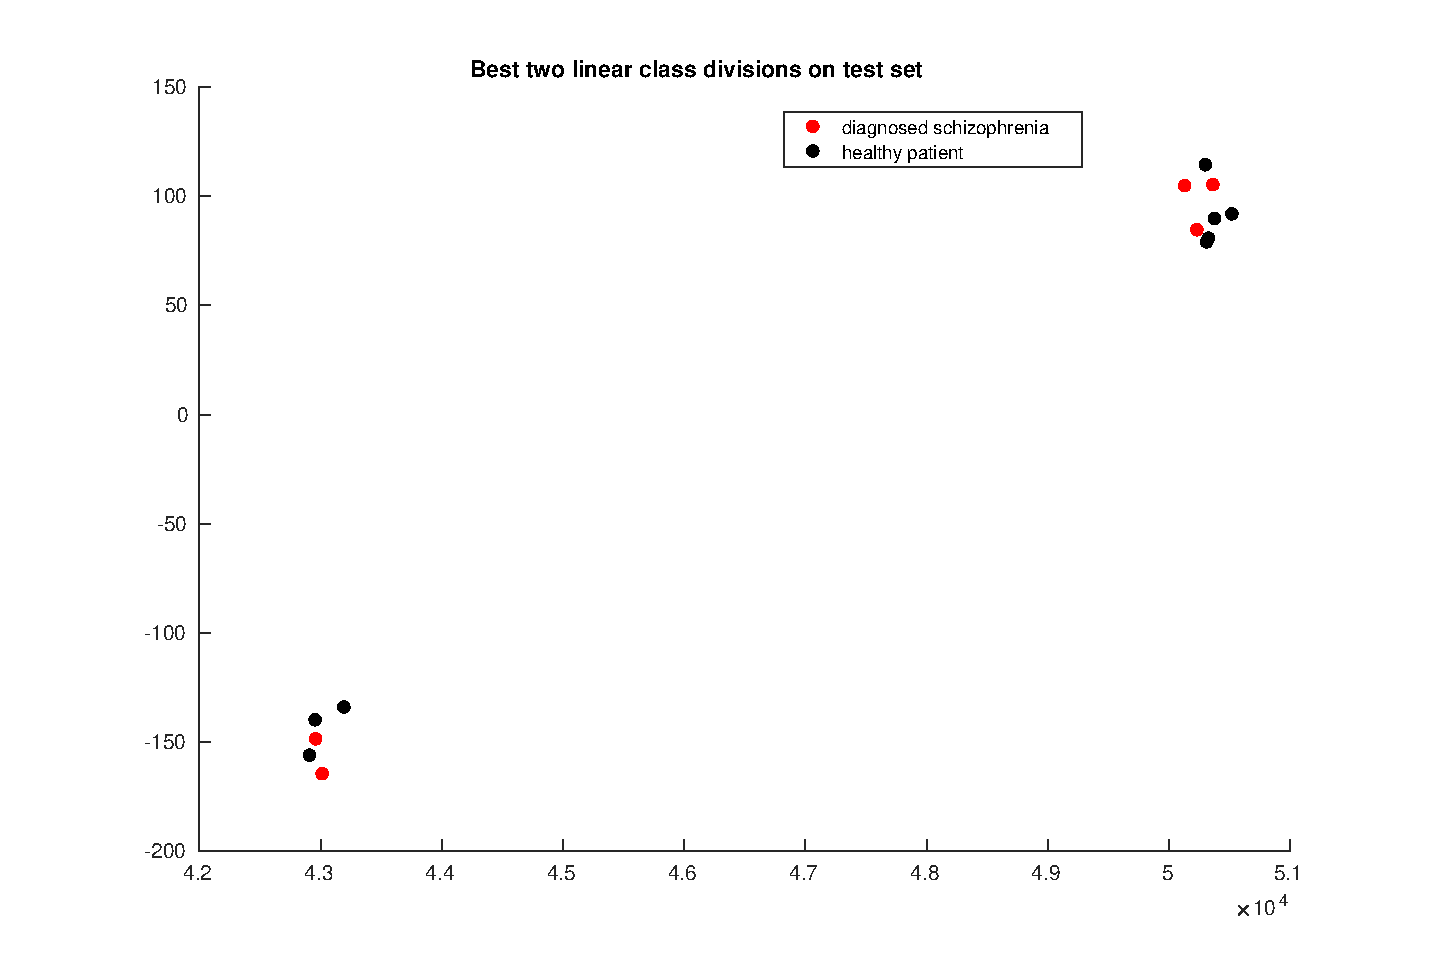
\includegraphics[width=0.9\linewidth, height=4cm]{Figures/LDA2DTest.eps}
        \caption{Best two linear separation on testing data}
    \end{subfigure}
 
    \caption{2D LDA}
\end{figure}

\subsection{LASSO}
For this section, MATLAB's built-in \verb!lasso! function was used to find a sparse weights matrix. Because the \verb!lasso! function provides several values of the penalty parameter $\lambda$ to choose from but does not utilize a good constant offset for easy classification, gradient descent was used to converge towards a more appropriate constant offset using the training data that would result in a lower error for the classification step. Running this routine several times through cross-validation, the mean value of $\lambda$ was 0.06, and the mean error rate on the validation set (a subset of the training set) was 24\%. The resultant vector of weights contains just 52 non-zero values, which is just $\approx 20\%$ of the total number of features. 

\subsection{Neural Networks with Gradient Descent}
A two-layer neural network that utilizes backpropagation for weight training was implemented. A sigmoid function was used as the activation function. After experimenting with several formulations of such a neural network, it was found that having both layers, each having 10 nodes and a constant offset, was able to give an error rate of 35\% when run on the testing data. This is not an unreasonable result considering the small training set that was used to train the network. The prediction labels are shown below.

\begin{figure}[H] 
    \centering
    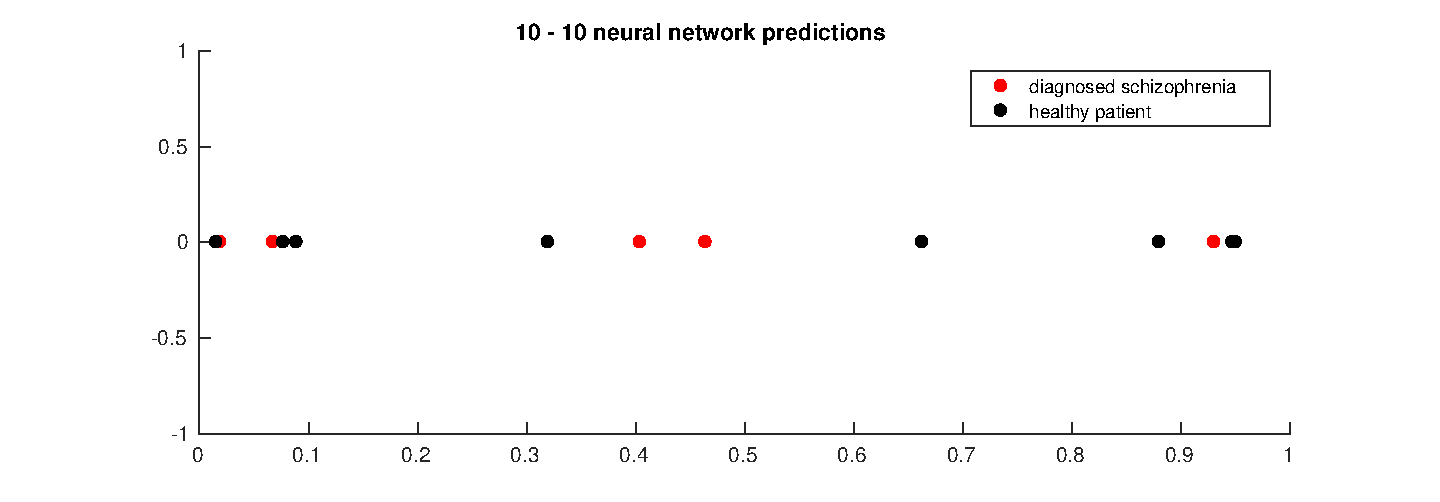
\includegraphics[width = \textwidth]{Figures/neuralnet.eps}
    \caption{Graphed output of trained neural net. Their positions on the horizontal axis determine how they would be classified, and their colors depict their true labels}
\end{figure}

%----------------------------------------------------------------------------------------
%	DISCUSSION
%----------------------------------------------------------------------------------------
\section{Discussion}
Beginning with LDA, the takeaway was that there was a separation between the two groups. This preliminary test showed that classification between the two groups was possible and so it was reasonable to continue.

Next, LASSO was attempted. Through the use of cross-validation and gradient descent, a model with reasonable predictive ability was achieved, especially taking into account the small initial dataset. Although LASSO took some processing and much verification, good results were achieved.

Finally, a neural network was trained on the data using gradient descent, but the results were unremarkable. One hypothesis for this would be that neural networks are not suited for such small amounts of training data, as it was not enough to make useful generalizations. While more data could have been extrapolated from given data, this was beyond the scope of the project. 

%----------------------------------------------------------------------------------------
%	CONCLUSION
%----------------------------------------------------------------------------------------
\section{Conclusion}
In the end, LASSO proved to be the best method of classification for this study. Although yet less useful for direct classification, LDA proved useful as a proof of possibility. The greatest hindrance for this analysis was the relatively small dataset provided by the Kaggle challenge, which was used for this report. 

With more data, it is likely that better classification would be possible due to better due to more constrained variables (i.e. a data matrix closer to being full-rank) and a wider range of more complex models such as neural networks. Cross-validation would have also have been more feasible without being detrimental to good results.

%----------------------------------------------------------------------------------------
%	REFERENCES
%----------------------------------------------------------------------------------------
\newpage
\section{References}
\printbibliography[heading=none]

\end{document}
